% ==========================================
% Session Info:
% System Prompt loaded: True
% History loaded: True
% 
% AI Studio User Prompt:
% [Dateien] 
% ==========================================

```latex
\section{Course Introduction and Logistics}

\begin{spoken-clean}[00:00:00 - 00:01:07]
Good morning. Good morning, thank you. Please, please, please. Uh, good morning and welcome to Analysis 2. Uh, I have here a projection with my name, Joaquim Serra, the name of the coordinator, Enric Florit-Simon. Now, this is my introduction. Um, and then you know the times of the lectures obviously because you are here. Um, and I wanted to share before starting with the mathematical content some practical informations that are very important because we are a large group and the communication and everything needs to be done in a more or less structured way, otherwise --- otherwise we collapse.

So, as I guess you did so as a general rule, uh, everything that applied to Analysis 1 applies to Analysis 2, unless otherwise stated. We will try to follow the same rules and then you know what to expect. In particular you will have this, uh, meta-for page \textit{[points at the projector screen]} that I can see that from from up there is a bit difficult to see, right? But I will try to put it bigger here.
\end{spoken-clean}

\begin{meta-note}[Projected Content: Course Website]
The lecturer displays the course website for \qt{Analysis II: mehrere Variablen Spring 2026}. It lists the lecturer (Joaquim Serra), coordinator (Enric Florit-Simon), lecture times (Mo 08:15-10:00 in ETA F 5, We 08:15-10:00 in HG F 7, Th 16:15-18:00 in ETA F 5), and information regarding exercise classes, communication via the Course Forum, recordings, and the final exam in August.
\end{meta-note}

\begin{spoken-clean}[00:01:07 - 00:02:55]
Um, so you know that you need to register for the exercise classes. Uh, for the communication, please try to use whenever possible the forum. We will look at the forum and and reply, and also your your peers can also reply to questions because many --- so then we can use the collective knowledge, right? Um, there will be recordings of the lecture, but not until the later on, okay? Because uh is important for the lecture and for you, but mainly --- I mean for you is your interest uh if you want to come or not, but for the lecture is very good that you come to the lecture, you ask questions, you stop me when I'm going too fast, these kind of things. You know, it's very important. So it's a --- and also is where you meet with your peers and you can communicate, ask questions to your peers. It's it's it's better for the learning.

Uh, we will tell you more about the exam later on, right? Today I will tell you a bit more what is important to be successful in the course, what to expect about this course, and uh the details and the rules of the exam will come later on. You don't need to know now. The bonus, there is a zero --- uh twenty-five bonus will be in questions that you will answer in some exercise classes. We will tell you in advance which ones, and uh essentially you need to be in the in the exercise class and answer it. And do not worry because uh the rule will be thought, in any case it's just $0.25$ points, uh but the rules will be thought so that if you miss one day or casuistics like this, it's not that you get zero points, right? Okay.
\end{spoken-clean}

\begin{spoken-clean}[00:02:55 - 00:04:15]
Uh, lecture notes. There will be lecture notes similar to those in Analysis 1, and we will put them in this page, hopefully by the end of each week, because I I update them after the lecture, mainly depending on your questions, depending on your feedback. And that's it. Uh, I think that the rules are mainly those and the organization. Is there some question uh about organization? So essentially as I said, um if you have doubts, uh is like in Analysis 1, unless I say something that is surprising to you as in Analysis 1. Is it okay, this? Yeah. Okay now, I will switch --- I have some other things I want to project later, but now because we cannot record at the same time blackboard and projection, I will switch one moment to the blackboard, so I can mute I think, yeah. Okay. Now we need the light. \textit{[The lecturer turns off the projector and prepares the blackboard]} Okay, I think that there is already on. Okay.
\end{spoken-clean}

\section{Analysis I vs. Analysis II: A Conceptual Overview}

\begin{spoken-clean}[00:04:15 - 00:05:30]
Okay now, just to start, um we will give a very quick --- so quick that it's almost a cartoon --- but a very quick overview of what is Analysis 1 and Analysis 2, right? It's very very quick. Analysis 1... is... sorry but for me it's very difficult to write big and then it's so --- so if you don't see something, I will try to say it out loud everything I write, but if if something --- I mean Analysis is a... so uh Analysis 1, calculus of one variable, right? 

And then if I if if we got to choose a representative theorem of Analysis 1, that a bit represents the course, uh what would you choose? So can you tell me, I know it's the first day, but let's start a bit of communication. Can you tell me at least two answers --- so two people can tell me what is the representative --- one representative theorem of Analysis 1? Yeah? \textit{[Student answers]} Yeah, I agree. Some other representative theorem --- he said the Fundamental Theorem of Calculus. Makes sense, right? Okay after --- is there some other guess? Is --- yeah, there? \textit{[Student answers]} The Intermediate Value Theorem. Okay.
\end{spoken-clean}

\begin{math-stroke}[The Fundamental Theorem of Calculus in 1D]
In Analysis I, the central object of study is the calculus of a single real variable.
\[
\text{Analysis 1: Calculus of One Variable}
\]
The most representative result is the \emph{Fundamental Theorem of Calculus} (FTC):
\begin{equation} \label{eq:ftc_1d}
\int_a^b f'(x) \, dx = f(b) - f(a)
\end{equation}

\begin{explanation-of-steps}
The lecturer initially writes $f(a) - f(b)$ on the board, but a student quickly spots the error. He corrects it to the standard $f(b) - f(a)$. He emphasizes that while the formula looks compact, understanding it required defining the derivative, the Riemann integral, and the structure of real numbers $\mathbb{R}$.
\end{explanation-of-steps}
\end{math-stroke}

\section{The Fundamental Theorem of Calculus in Higher Dimensions}

\begin{spoken-clean}[00:05:30 - 00:06:23]
I think we need to use this for the recording otherwise I will repeat. Later on when I get better with the throwing the \textit{[referring to the catch-box microphone]} we will use that. So, okay, so fundamental --- so we we said two theorems that are um that are indeed important. Perhaps the most representative I would agree and and I saw many people saying yes, so it's the Fundamental Theorem of Calculus, right? And it's this \textit{[points at Equation \ref{eq:ftc_1d}]}. Is it correct? Yeah, looks like, no?

Now, to to unfold and to write and to understand every detail about this equation over here, you needed to introduce a lot of things. You needed to define what is that (i.e., the derivative $f'(x)$), right? What is this (i.e., the integral $\int_a^b \dots dx$)? And even --- and you spent a lot of time, right? What is that (i.e., the real number $\mathbb{R}$)? It was not --- it was not easy. Yeah, there is some mistake? \textit{[Corrects the board]} Good, well spotted. $f(b) - f(a)$. Now? 

Okay so this is a fairly compact theorem, yet the ingredients you had to learn to unfold all of this and to understand the meaning of every symbol here were a bit of work. Now, how will Analysis 2 look like? So this will be calculus, still calculus, in uh more than one variable. Well, since you already know one, let's say at least two variables, because otherwise it's already covered by Analysis 1.
\end{spoken-clean}

\begin{math-stroke}[Preview: The Fundamental Theorem in Higher Dimensions]
Analysis II extends these concepts to multiple variables, typically in $\mathbb{R}^n$.
\[
\text{Analysis 2: Calculus in } \ge 2 \text{ Variables}
\]
The higher-dimensional counterparts to the FTC are known by various names:
\begin{itemize}
    \item Gauss's Theorem
    \item Stokes's Theorem
    \item Divergence Theorem
    \item Green's Theorem
\end{itemize}

\begin{center}
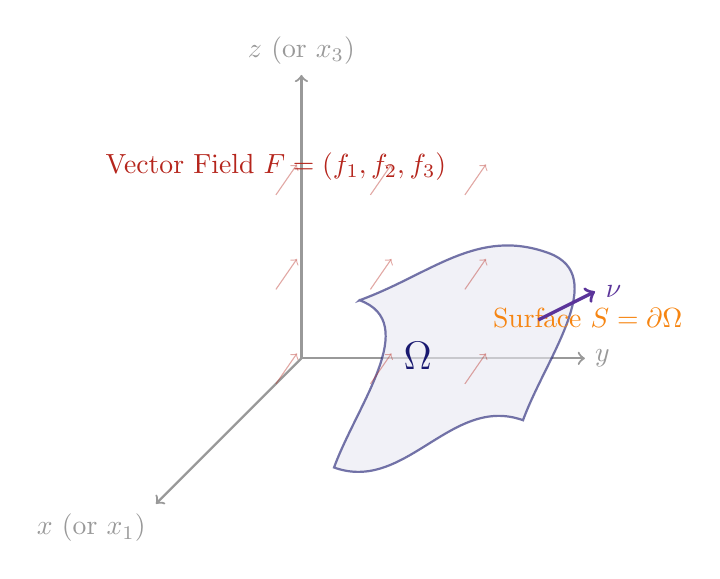
\begin{tikzpicture}[scale=1.2]
    % This TikZ diagram is extracted from the blackboard at 00:09:30
    % 3D Axes
    \draw[->, thick, gray!80] (0,0,0) -- (3,0,0) node[right] {$y$};
    \draw[->, thick, gray!80] (0,0,0) -- (0,3,0) node[above] {$z$ (or $x_3$)};
    \draw[->, thick, gray!80] (0,0,0) -- (0,0,4) node[below left] {$x$ (or $x_1$)};

    % The "Potato" Domain Omega
    \draw[thick, MidnightBlue, fill=MidnightBlue!10, opacity=0.6] 
        (1,1,1) to[out=20,in=160] (3,1.5,1) 
        to[out=-20,in=70] (3.5,0.5,3) 
        to[out=160,in=-20] (1.5,0,3) 
        to[out=70,in=-20] cycle;
    \node[MidnightBlue] at (2,0.8,2) {\Large $\Omega$};
    
    % The Surface S (The "Skin")
    \node[BurntOrange] at (3.8,1.2,2) {Surface $S = \partial \Omega$};
    
    % Vector Field F (The "Cereal Field")
    \foreach \x in {0.5, 1.5, 2.5}
        \foreach \y in {0.5, 1.5, 2.5}
            \draw[->, BrickRed, opacity=0.4] (\x,\y,2) -- (\x+0.3, \y+0.4, 2.2);
    \node[BrickRed] at (0.5, 2.8, 2) {Vector Field $F = (f_1, f_2, f_3)$};

    % Normal Vector nu
    \draw[->, very thick, RoyalPurple] (3.2, 1.1, 1.8) -- (3.8, 1.4, 1.8) node[right] {$\nu$};
\end{tikzpicture}
\end{center}

The generalized theorem relates the integral of a derivative over a volume to the flux across its boundary:
\begin{equation} \label{eq:ftc_nd}
\underbrace{\int_{\Omega} \sum_{i=1}^n \frac{\partial f_i}{\partial x_i} \, dx}_{\text{Integral of "Derivative" over Volume}} = \underbrace{\int_{S} F \cdot \nu \, dS}_{\text{Flux across Boundary Surface}}
\end{equation}
\end{math-stroke}

\begin{spoken-clean}[00:06:23 - 00:07:45]
And some representative theorem that would be the equivalent, so the counterpart of this one, is the Gauss --- it has many names and it's always the same theorem, so but --- so it's the Gauss, Stokes, uh Divergence, sometimes it's called the Divergence Theorem, uh and that's it, I think Green, sometimes Green Theorem. 

And now I will write the theorem and you will not understand exactly what each thing means, I will tell you intuitively, and then the goal of the lecture will be at the end of the lecture you will be able to understand in full precision everything that I wrote here. Okay? So the theorem goes as follows. So we have --- we have the space, the space, let's say I will put it in the space $\mathbb{R}^3$. Three coordinates of space, right? This thing: $x, y, z$ or $x_1, x_2, x_3$. Sometimes $x_1, x_2, x_3$. Right? 

And then in the --- in this space we are given a domain, we are given some or some surface that encloses some interior, so this --- this is the interior of the surface and the exterior. And this is a surface. Right? The surface I call it $S$. What is a surface? It could be a sphere, it could be a sort of the \qt{skin of a potato}. It's a surface. Two-dimensional object. It has and --- and what I'm --- this kind of surface will have a interior and exterior, and the interior of the surface, so the --- if the surface is the skin of the potato, the --- the filling of the potato, the white part, right? is $\Omega$, I call it $\Omega$.
\end{spoken-clean}

\begin{didactic-insight}[The Potato Analogy]
The lecturer uses the \qt{potato} analogy to ground abstract topological concepts. The \qt{skin} represents the 2D boundary surface $S$, while the \qt{filling} represents the 3D interior volume $\Omega$. This physical metaphor helps students visualize the relationship between a set and its boundary in higher dimensions.
\end{didactic-insight}

\begin{spoken-clean}[00:07:45 - 00:09:01]
And then the equivalent of this theorem in this setup is this: Given a vector field --- now you don't know what it is a vector field, let me tell you, $F = (f_1, f_2, f_3)$. These are three --- three functions of space, right? At each point of space you have three numbers. Here you have three numbers, here you have three numbers, yeah. This is a vector field $F$. And how we do we draw vector fields? Uh, we draw it like this, right? It's like a --- a field of some cereal, right? but in every point you have an arrow instead of a --- a plant. 

Okay, so this is the vector field $F$. And the theorem says that the integral in $\Omega$ of the derivative of the field, the $i$-component with respect to the $x_i$ variable, and you sum over $i$, this is equal to the flux of the field across the boundary, across the $S$. And it's called like this: $\int_S F \cdot \nu \, dS$. This is the same theorem you have got here in one dimension, in several variables.
\end{spoken-clean}

\begin{spoken-clean}[00:09:01 - 00:10:45]
Now, the small problem is that maybe some of you in physics or --- or in previous courses have seen some of this notation, probably not, I don't expect you to --- we --- and we will need to introduce each of these notations. These partial derivatives, what is a domain, what is a surface? What is this surface mathematically? How do you model a surface? How do you compute a integral over a surface? You know how to compute a integral over the real line, right? over a segment, but over a surface? This will need some definition and some work. And these objects that are the partial derivatives. 

So here in --- in one equation you have a bit the goal and the syllabus of the course. How will --- how will we proceed? So first we will start looking at the space. In Analysis 1 you did everything in $\mathbb{R}$. Now we will need to introduce $\mathbb{R}^3$, but we are mathematicians so we will --- well, some of us. Uh, some of you are physicist or are proto-physicist, would like to become physicist. So we will use this because we don't want to spend time proving the same theorem in --- in the plane $\mathbb{R}^2$, then in $\mathbb{R}^3$ in the space, and then when you go to do general relativity you need $\mathbb{R}^4$, right? We do everything in $\mathbb{R}^n$. $n$ is the dimension.
\end{spoken-clean}

\begin{spoken-clean}[00:10:45 - 00:11:00]
So what is $\mathbb{R}^n$? Is the set of $n$-tuples of real numbers. This is the definition, okay? And what is this? This is the same as the set of points we will denote a point $x$, but now $x$ will carry $n$ coordinates: $x_1, x_2, \dots, x_n$. Now this is the point. And these $x_i$ are real numbers. This you know probably because you are doing well or you have done linear algebra, right? So this should be quite familiar. But still it's good that we recall. Okay.
\end{spoken-clean}

[SYSTEM] Segment complete. Please prompt "Continue" for the remainder of the segment.```